\documentclass[10pt,a4paper]{article}

\usepackage[utf8]{inputenc}
\usepackage[french]{babel}
\usepackage[T1]{fontenc}
\usepackage{amsmath}
\usepackage{amsfonts}
\usepackage{amssymb}
\usepackage{hyperref}
\usepackage{graphicx}
\usepackage{caption}
\usepackage{subcaption}
\usepackage[left=2cm,right=2cm,top=2cm,bottom=2cm]{geometry}

\title{Journal de bord}
\author{Gabin Serrurot}

\begin{document}

\maketitle

\section{Journal de bord}

\begin{enumerate}
    \item \textbf{08/01/2024:}
        \begin{itemize}
            \item J'ai lu le dossier de présentation du projet
            \item J'ai essayé de créer une organisation sur Github afin d'avoir tous les codes au même endroit et afin d'éviter d'être dépend les uns des autres
        \end{itemize}
    \item \textbf{09/01/2024:}
        \begin{itemize}
            \item J'ai finalement décidé de ne pas faire une organisation, juste de faire un dossier dans mon compte Github et accorder l'accès à Yahya et Andréa afin de tout simplifier. De cette manière, je peux utiliser Github Desktop
            \item J'ai commencé le diagramme des cas d'utilisation "Aller à la recherche d’un actif dans l’entrepôt" avec le site \href{https://online.visual-paradigm.com}{visual-paradigm} : figure~\ref{recherche-actif.png1}
            \item J'ai commencé le diagramme des cas d'utilisation "Contrôler le chargement du camion" avec le site \href{https://online.visual-paradigm.com}{visual-paradigm} : figure~\ref{controle-chargement.png1}
            \item Il y aura aussi les diagrammes d'exigences et de déploiement à faire, même s'ils ne sont pas notés dans le dossier de présentation du projet
        \end{itemize}
    \item \textbf{10/01/2024:}
        \begin{itemize}
            \item J'ai d'abord perdu une bonne heure à essayer de debugger mon journal de bord, l'inclusion d'images ne fonctionnait pas alors qu'il manquait juste "usepackage{graphicx}" pour que tout fonctionne.
            \item J'ai repris les diagrammes que j'ai fais la veille avec M. Hacquard : figures~\ref{recherche_actif.png2} et~\ref{controle_chargement.png2} 
        \end{itemize}
    \item \textbf{11/01/2024:}
        \begin{itemize}
            \item Je me suis lancé dans les diagrammes de déploiement mais Pierre m'a dit que ces diagrammes sont à faire par équipe car ils représentent tout le système, pas chacun le sien
            \item J'ai donc décidé de faire la reformulation du cahier des charges
        \end{itemize}
    \item \textbf{12/01/2024:}
        \begin{itemize}
            \item J'ai vu pour la première fois un beacon avec M. Lejoncour
            \item J'ai commencé le cahier de recettes
        \end{itemize}
    \item \textbf{15/01/2024:}
        \begin{itemize}
            \item J'ai fais l'IHM de l'application (la veille mais faut pas le dire, cf image~\ref{idee_design_application1})
            \item J'ai continué le cahier de recettes
            \item J'ai aidé Andréa à installer \textbf{JMerise}
            \item "Définir le plan de numérotation des tags" devient "Donner un tableau exemple d'association entre les beacons et les actifs" dans \textbf{Planification des tâches du projet}
        \end{itemize}
    \item \textbf{16/01/2024:}
        \begin{itemize}
            \item Avec Yahya et Andréa nous avons fait le diagramme de déploiement (cf image~\ref{diagramme_deploiement}) et le diagramme d'exigences  (cf image~\ref{diagramme_exigences1})
            \item Le diagramme de déploiement convient bien mais par le diagramme d'exigences
            \item Pour l'IHM, je ne ferai probablement pas de système de connexion car ça rajouterait des contraintes trop importantes en terme de charge de travail, je me contenterai probablement plus d'un bouton de type "switch" pour basculer entre le mode de contrôle du chargement et le mode de recherche d'actif dans l'entrepôt
        \end{itemize}
    \item \textbf{17/01/2024:}
        \begin{itemize}
            \item Nous allons reprendre le diagramme d'exigences. En parlant avec M. Hacquard, nous avons fait deux diagrammes d'exigences, un pour le camion (cf image~\ref{diagramme_exigences_camion}) et un pour l'entrepôt (cf image~\ref{diagramme_exigences_entrepot})
            \item Nous avons également légèrement modifié le diagramme de déploiement (cf image~\ref{diagramme_deploiement2})
        \end{itemize}
    
    \newpage
    
    \item \textbf{18/01/2024:}
        \begin{itemize}
            \item Je vais commencer mes fiches de test car M. Hacquard a dit que les exigences en périphérie du diagramme d'exigences représentent les tests unitaires et les exigences plus hautes dans la hiérarchie du diagramme représentent les tests d'intégration
            \item J'ai réagencer le diagramme d'exigences de l'entrepôt pour améliorer la lisibilité
            \item J'ai perdu énormément de temps car \textbf{Github Desktop} a fait des siennes, il ne m'affichait plus les commits donc je ne pouvais pas faire de push sur mon Github. Je suis sorti de la salle sans que le problème soit résolu, espérons que ça ira mieux demain
        \end{itemize}
    \item \textbf{19/01/2024:}
        \begin{itemize}
            \item A priori Github Desktop fonctionne de nouveau, j'ai quand même pris du temps pour reprendre là où jen étais hier
            \item On a convenu avec M. Le Joncour que nous feront notre première revue non formelle vendredi prochain, le 26 janvier donc il faudra que nous fassions notre diapo lundi ou mardi prochain afin d'être pret en avance. Il s'agit d'une revue non formelle donc il n'y aura normalement pas de partie individuelle, il y a juste la présentation en groupe à faire. Pour cette revue nous attendons que Andréa et Yahya aient finis le modèle logique de données
            \item J'ai réalisé le cahier plan de numérotation des tags
            \item J'ai poursuivi les fiches de tests
        \end{itemize}
    \item \textbf{20/01/2024:}
        \begin{itemize}
            \item J'ai terminé (sur mon temps libre oui) les fiches de tests
        \end{itemize}
    \item \textbf{22/01/2024:}
        \begin{itemize}
            \item J'étais en CCF, je n'ai rien pu faire du tout je suis sorti 10 minutes avant la fin
        \end{itemize}
    \item \textbf{23/01/2024:}
        \begin{itemize}
            \item Nous avons d'abord décidé de ce que nous allions mettre dans nos diapos
        \end{itemize}
    \item \textbf{11/01/2024:}
        \begin{itemize}
            \item 
        \end{itemize}
\end{enumerate}

\newpage

\section{Annexes}

\begin{figure}[h!]
    \centering
    \begin{subfigure}[b]{0.45\textwidth}
        \centering
        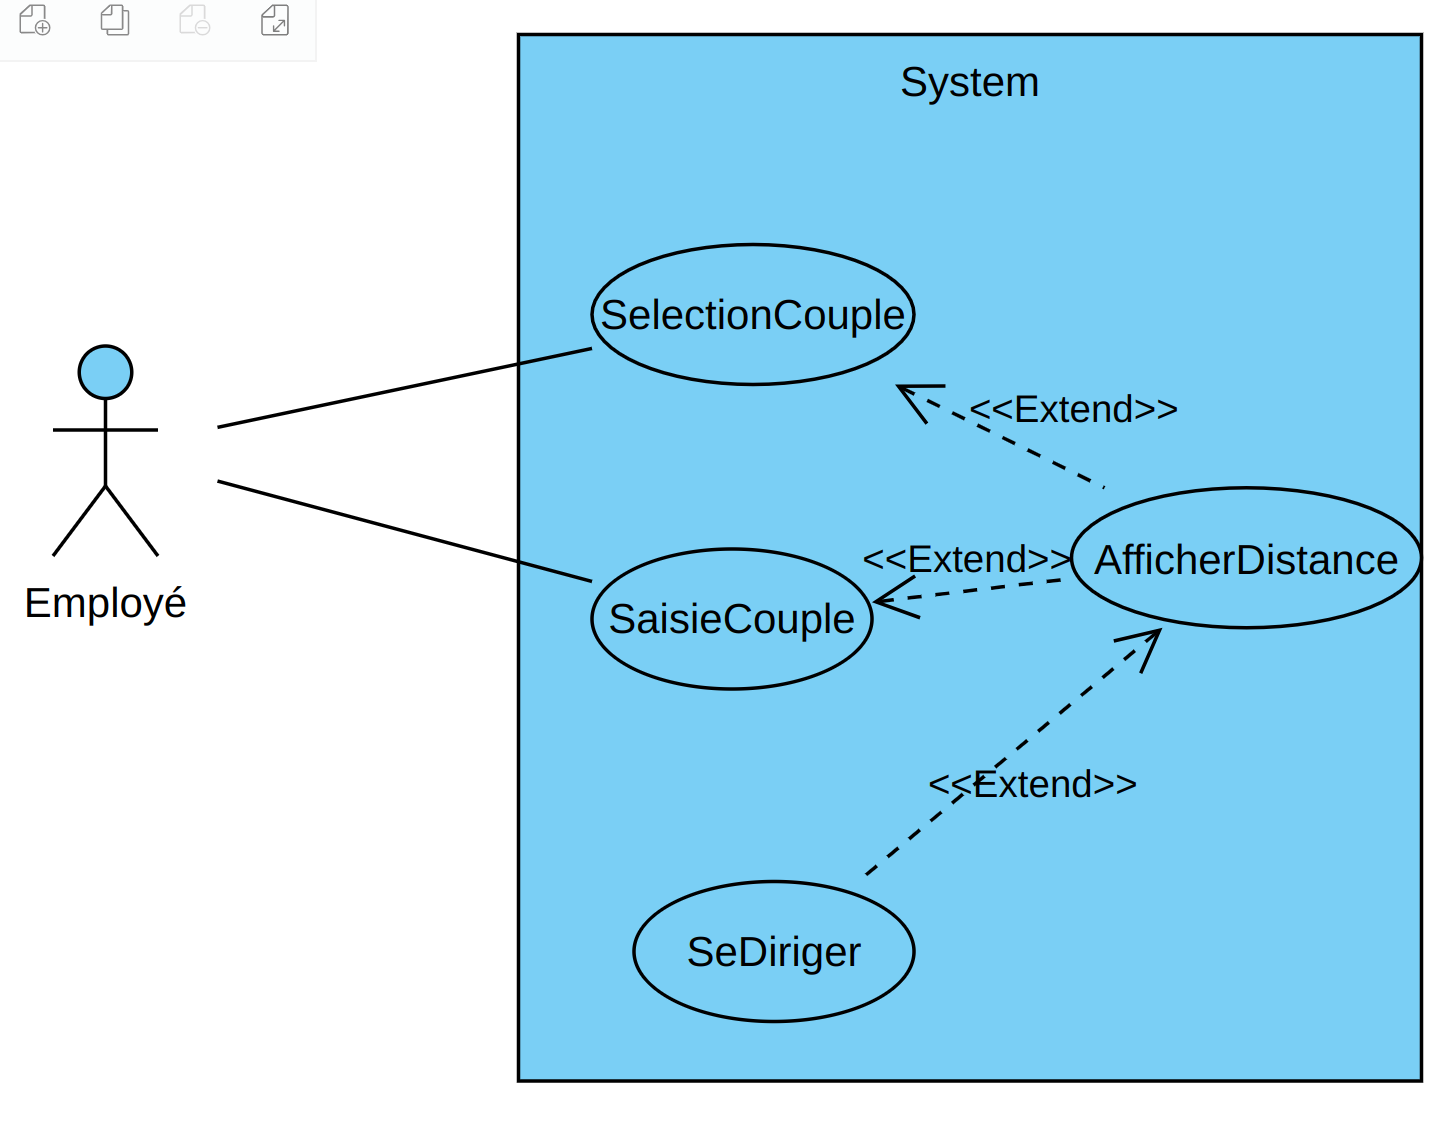
\includegraphics[scale=0.14]{Images/recherche-actif.png}
        \caption{}
        \label{recherche-actif.png1}
    \end{subfigure}
    \begin{subfigure}[b]{0.45\textwidth}
        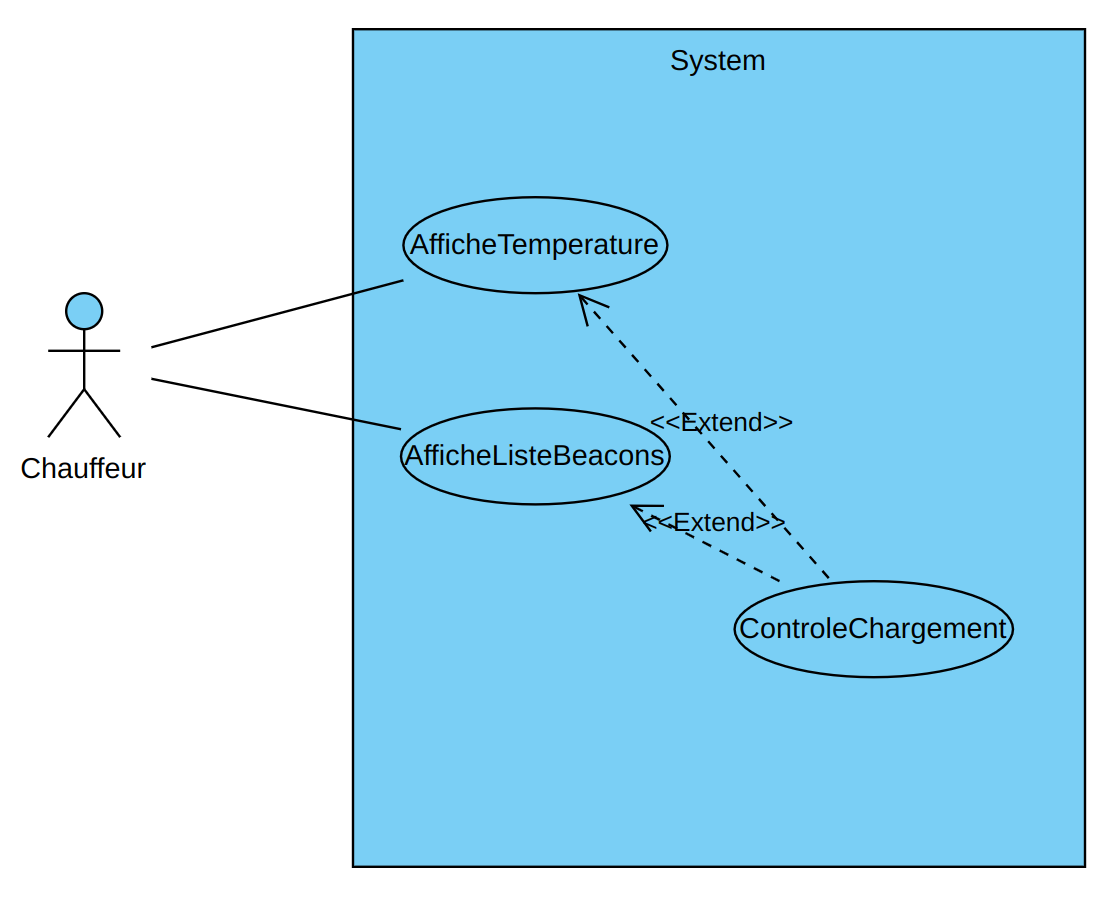
\includegraphics[scale=0.14]{Images/controle-chargement.png}
        \caption{}
        \label{controle-chargement.png1}
    \end{subfigure}
    \caption{}
\end{figure}

\begin{figure}[h!]
    \centering
    \begin{subfigure}[b]{0.45\textwidth}
        \centering
        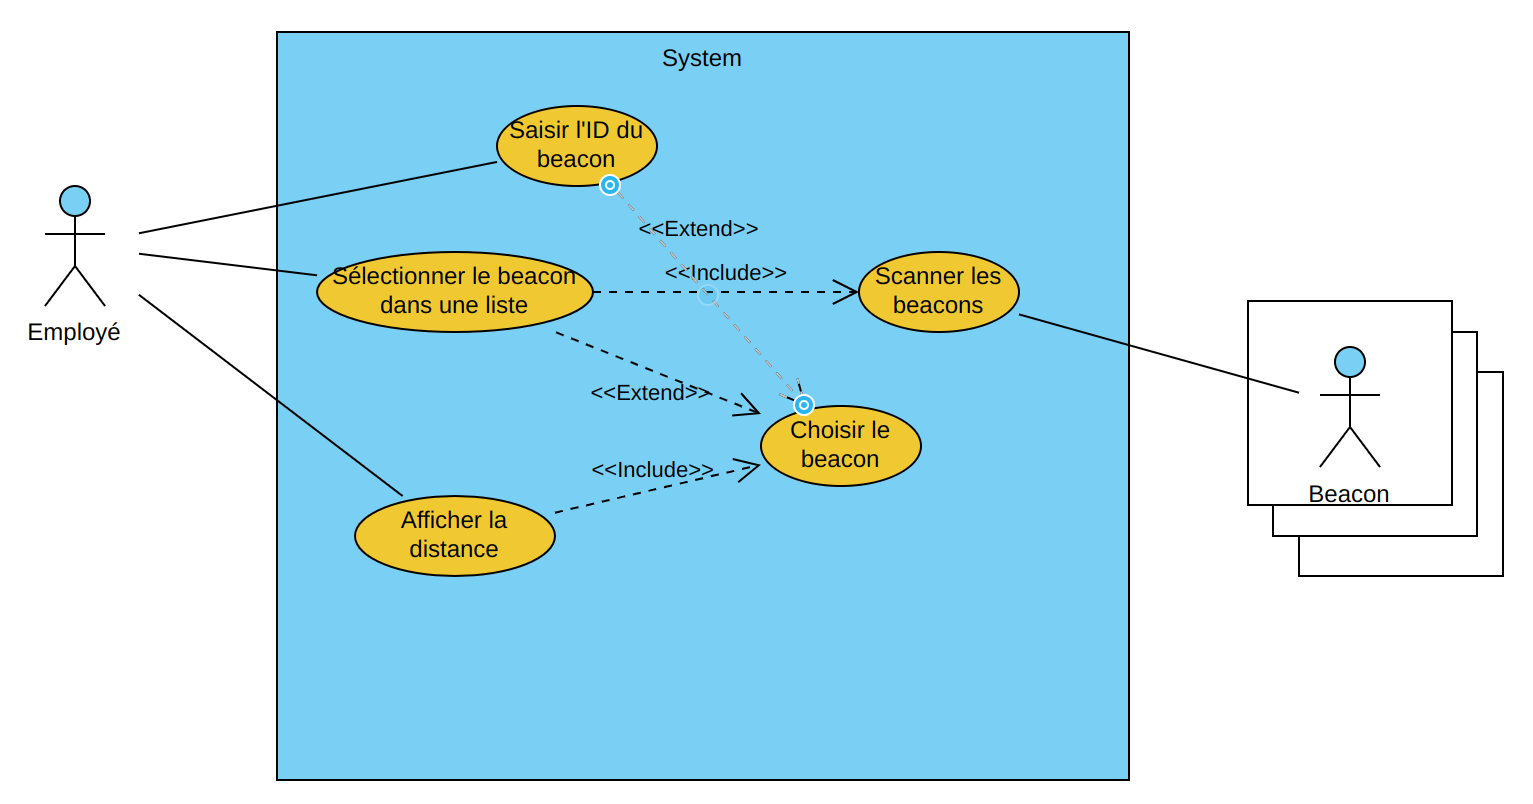
\includegraphics[scale=0.14]{Images/recherche_actif.png}
        \caption{}
        \label{recherche_actif.png2}
    \end{subfigure}
    \begin{subfigure}[b]{0.45\textwidth}
        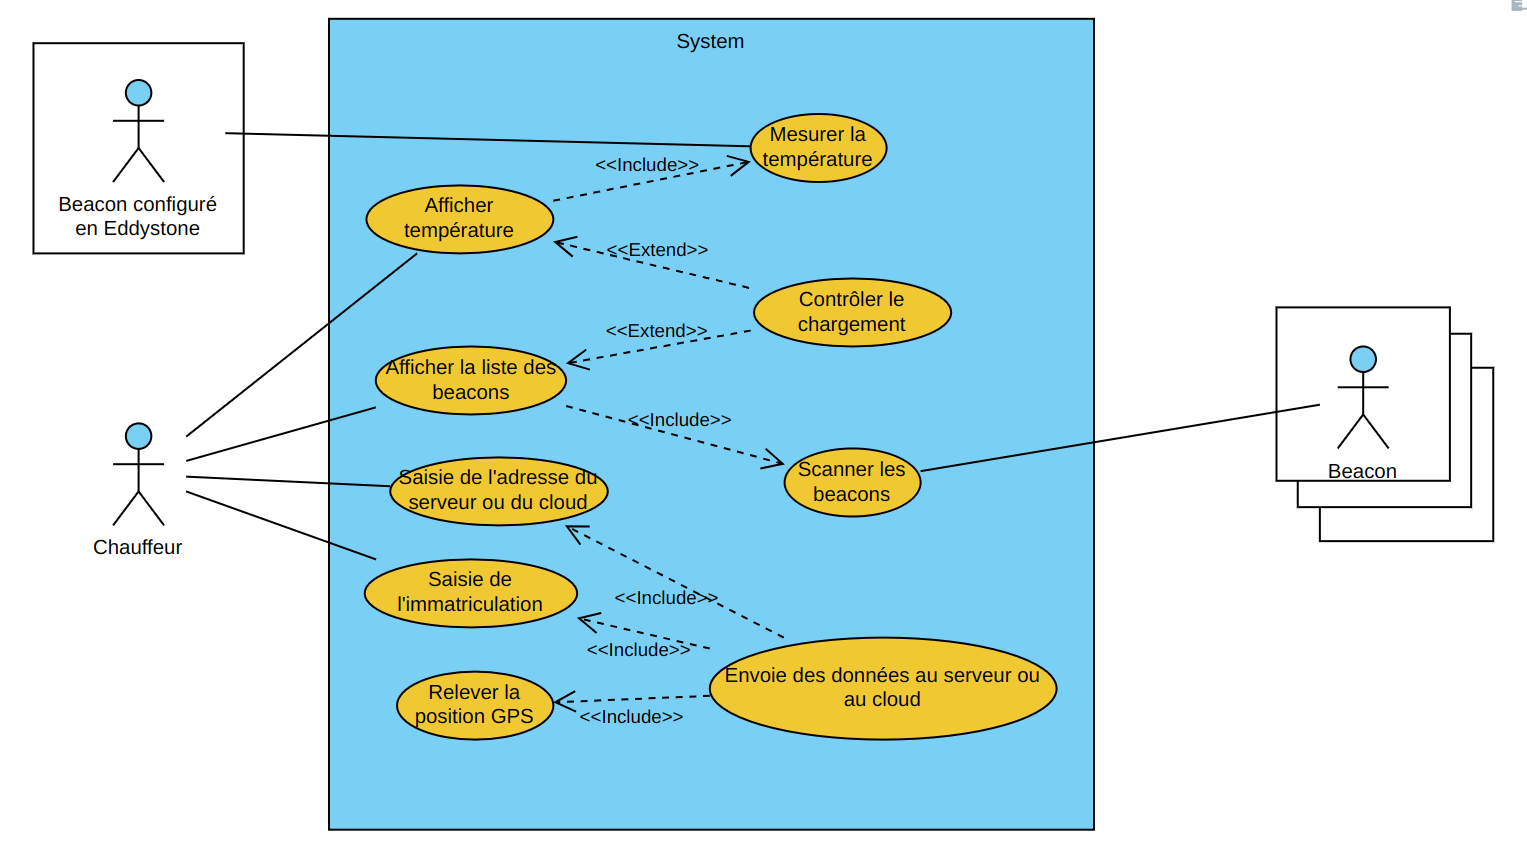
\includegraphics[scale=0.14]{Images/controle_chargement.png}
        \caption{}
        \label{controle_chargement.png2}
    \end{subfigure}
    \caption{}
\end{figure}

\begin{figure}[h!]
    \centering
    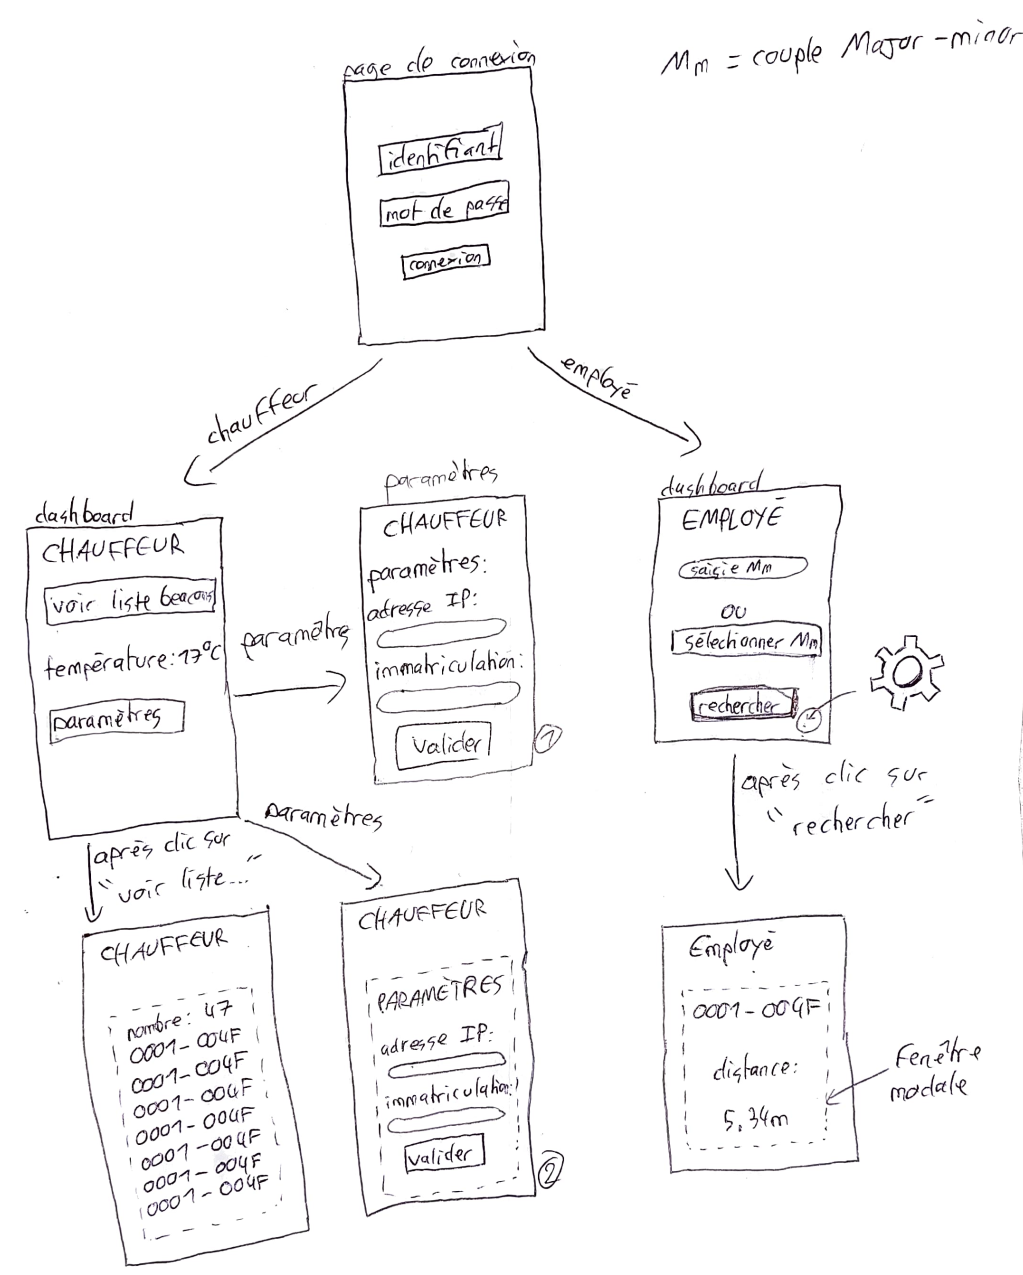
\includegraphics[scale=0.2]{Images/idee_design_application1.png}
    \caption{}
    \label{idee_design_application1}
\end{figure}

\begin{figure}[h!]
    \centering
    \begin{subfigure}[b]{0.45\textwidth}
        \centering
        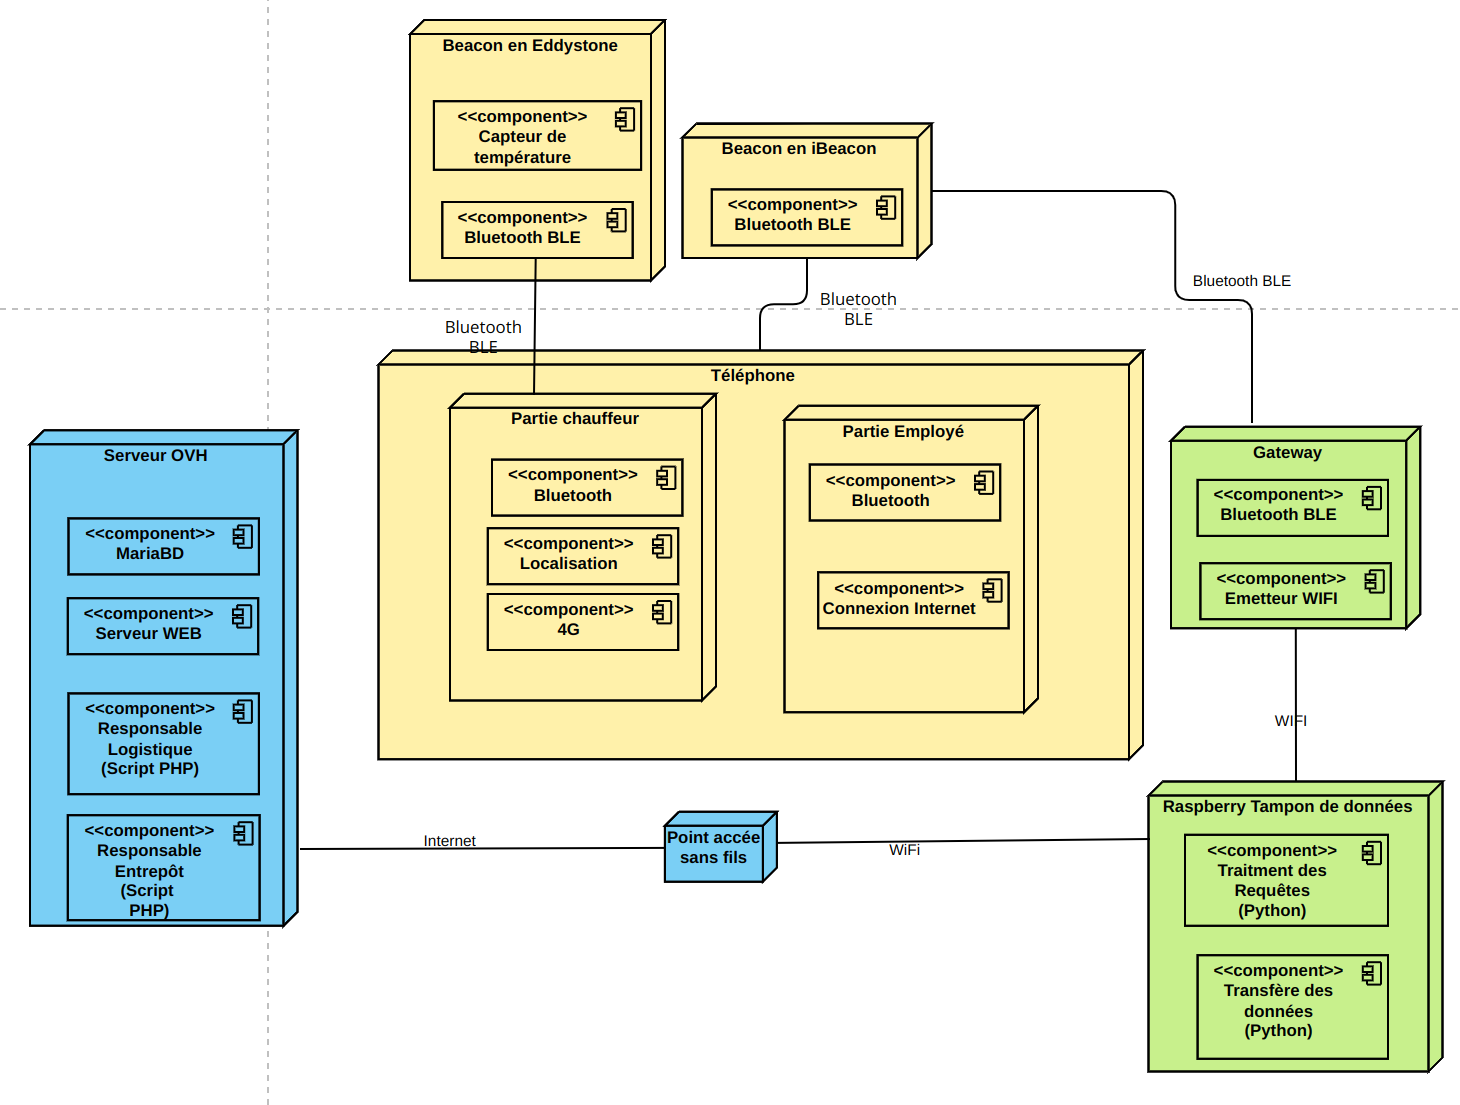
\includegraphics[scale=0.14]{Images/diagramme_deploiement.png}
        \caption{}
        \label{diagramme_deploiement}
    \end{subfigure}
    \begin{subfigure}[b]{0.45\textwidth}
        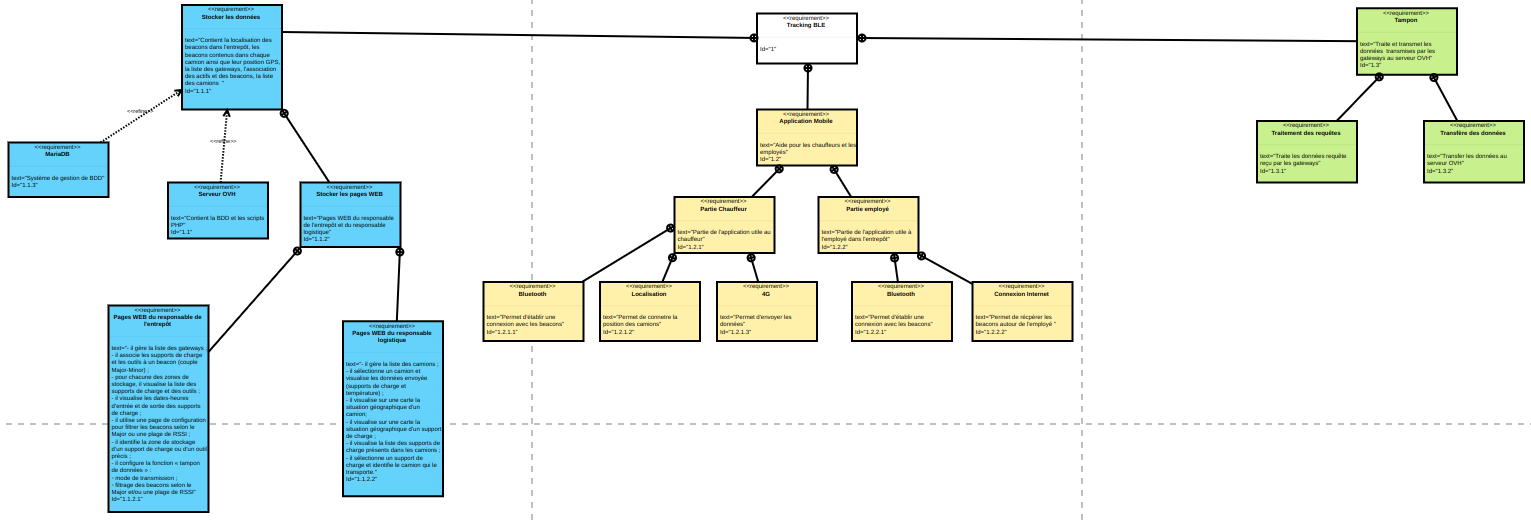
\includegraphics[scale=0.14]{Images/diagramme_exigence1.png}
        \caption{}
        \label{diagramme_exigences1}
    \end{subfigure}
    \caption{}
\end{figure}

\begin{figure}[h!]
    \centering
    \begin{subfigure}[b]{0.45\textwidth}
        \centering
        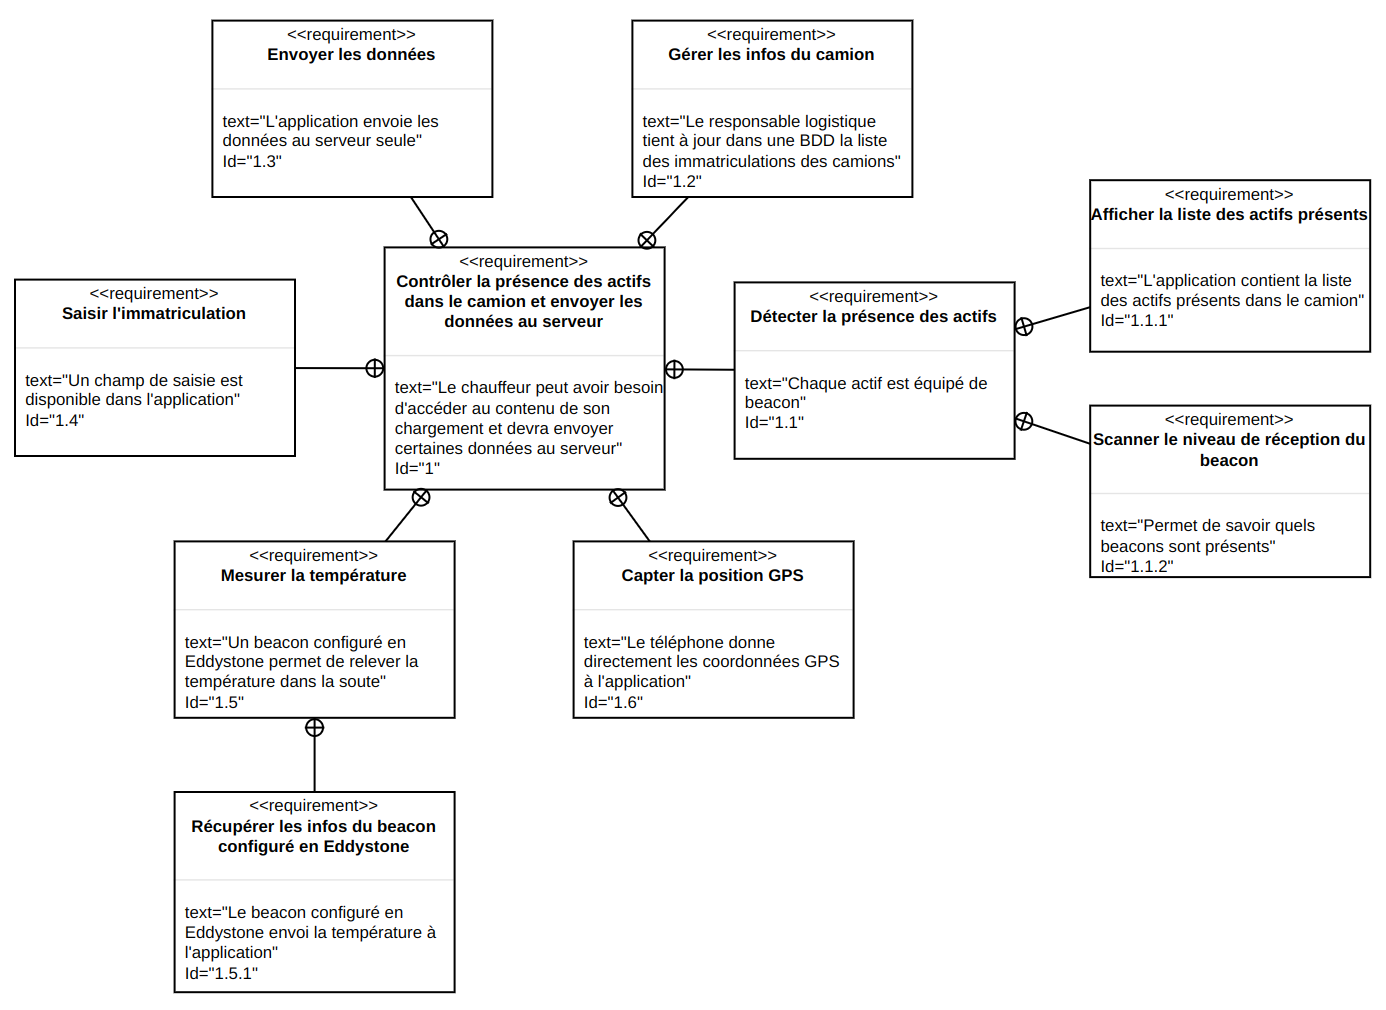
\includegraphics[scale=0.14]{Images/diagramme_exigences_camion.png}
        \caption{}
        \label{diagramme_exigences_camion} 
    \end{subfigure}
    \begin{subfigure}[b]{0.45\textwidth}
        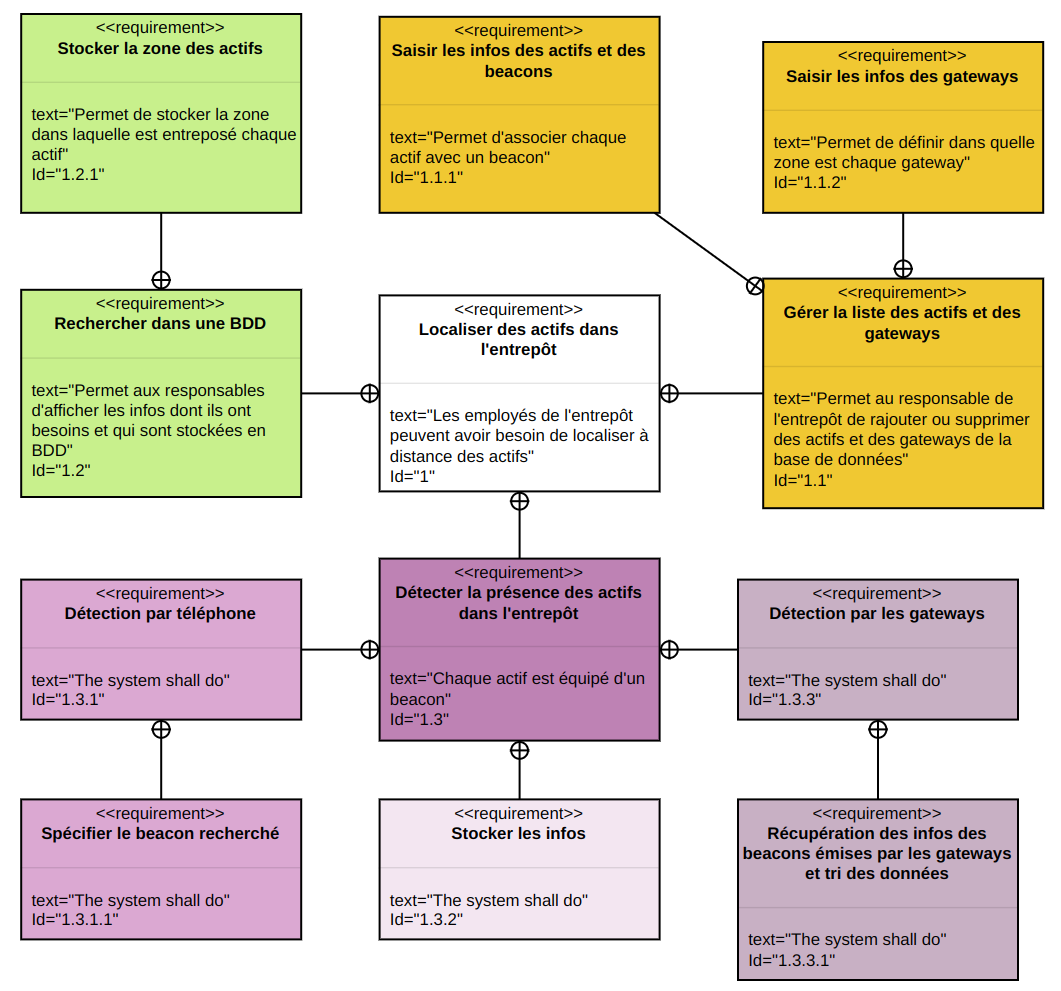
\includegraphics[scale=0.14]{Images/diagramme_exigences_entrepot.png}
        \caption{}
        \label{diagramme_exigences_entrepot}
    \end{subfigure}
    \caption{}
\end{figure}

\begin{figure}[h!]
    \centering
    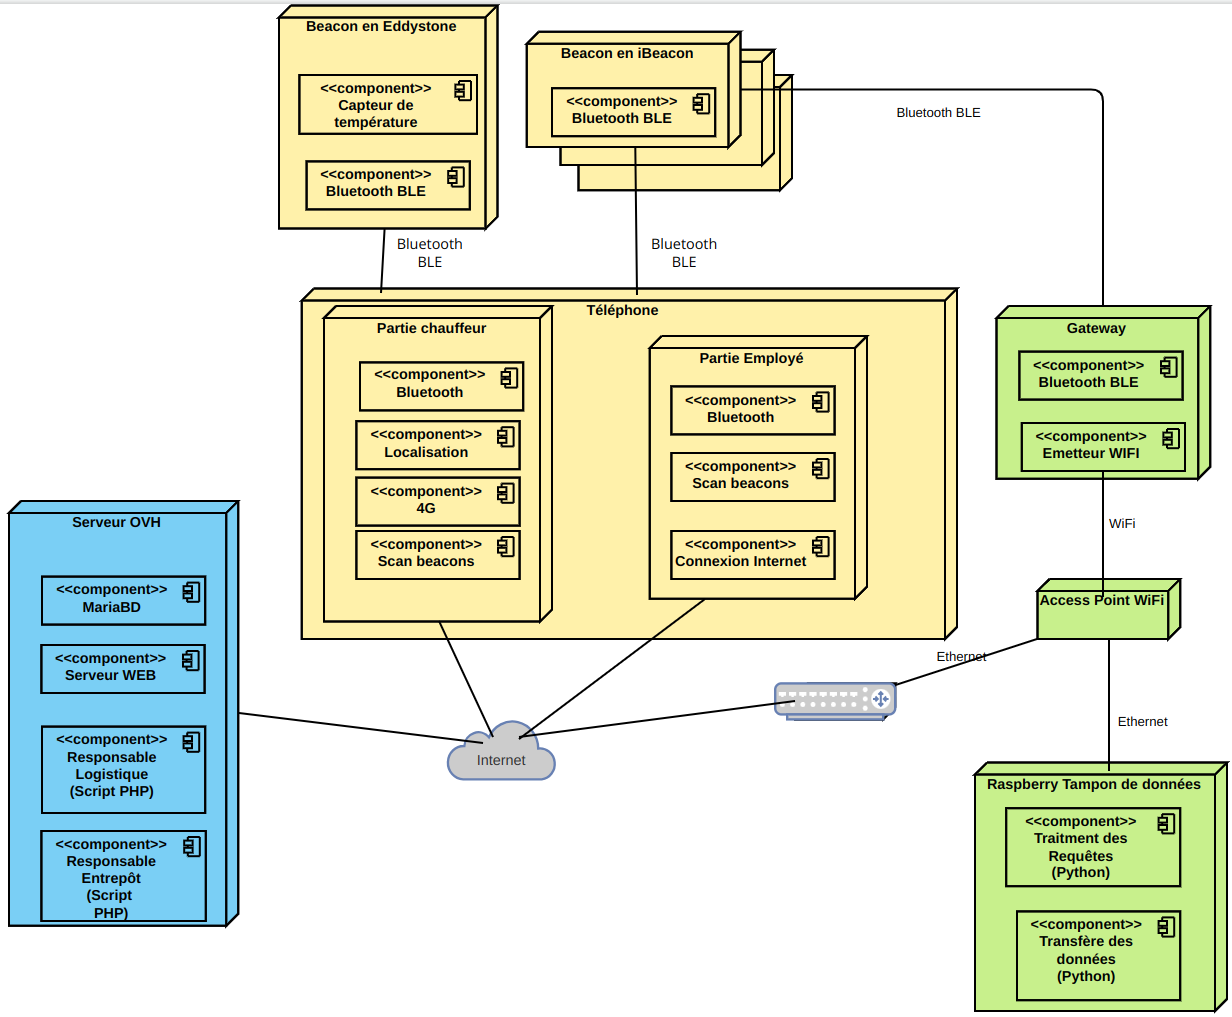
\includegraphics[scale=0.2]{Images/diagramme_deploiement2.png}
    \caption{}
    \label{diagramme_deploiement2}
\end{figure}

\end{document}
